%!TEX root = ../main.tex
\begin{frame}{The Optimal Control Problem}
    \setlength{\leftmargini}{1mm}
    \begin{textblock*}{130mm}(0mm, 20mm)
        \only<1>{

            \includegraphics[scale=0.125,%
                keepaspectratio]{assets/%
                SchemeModel_withoutVaccination01.png}
        }
        \only<2>{
            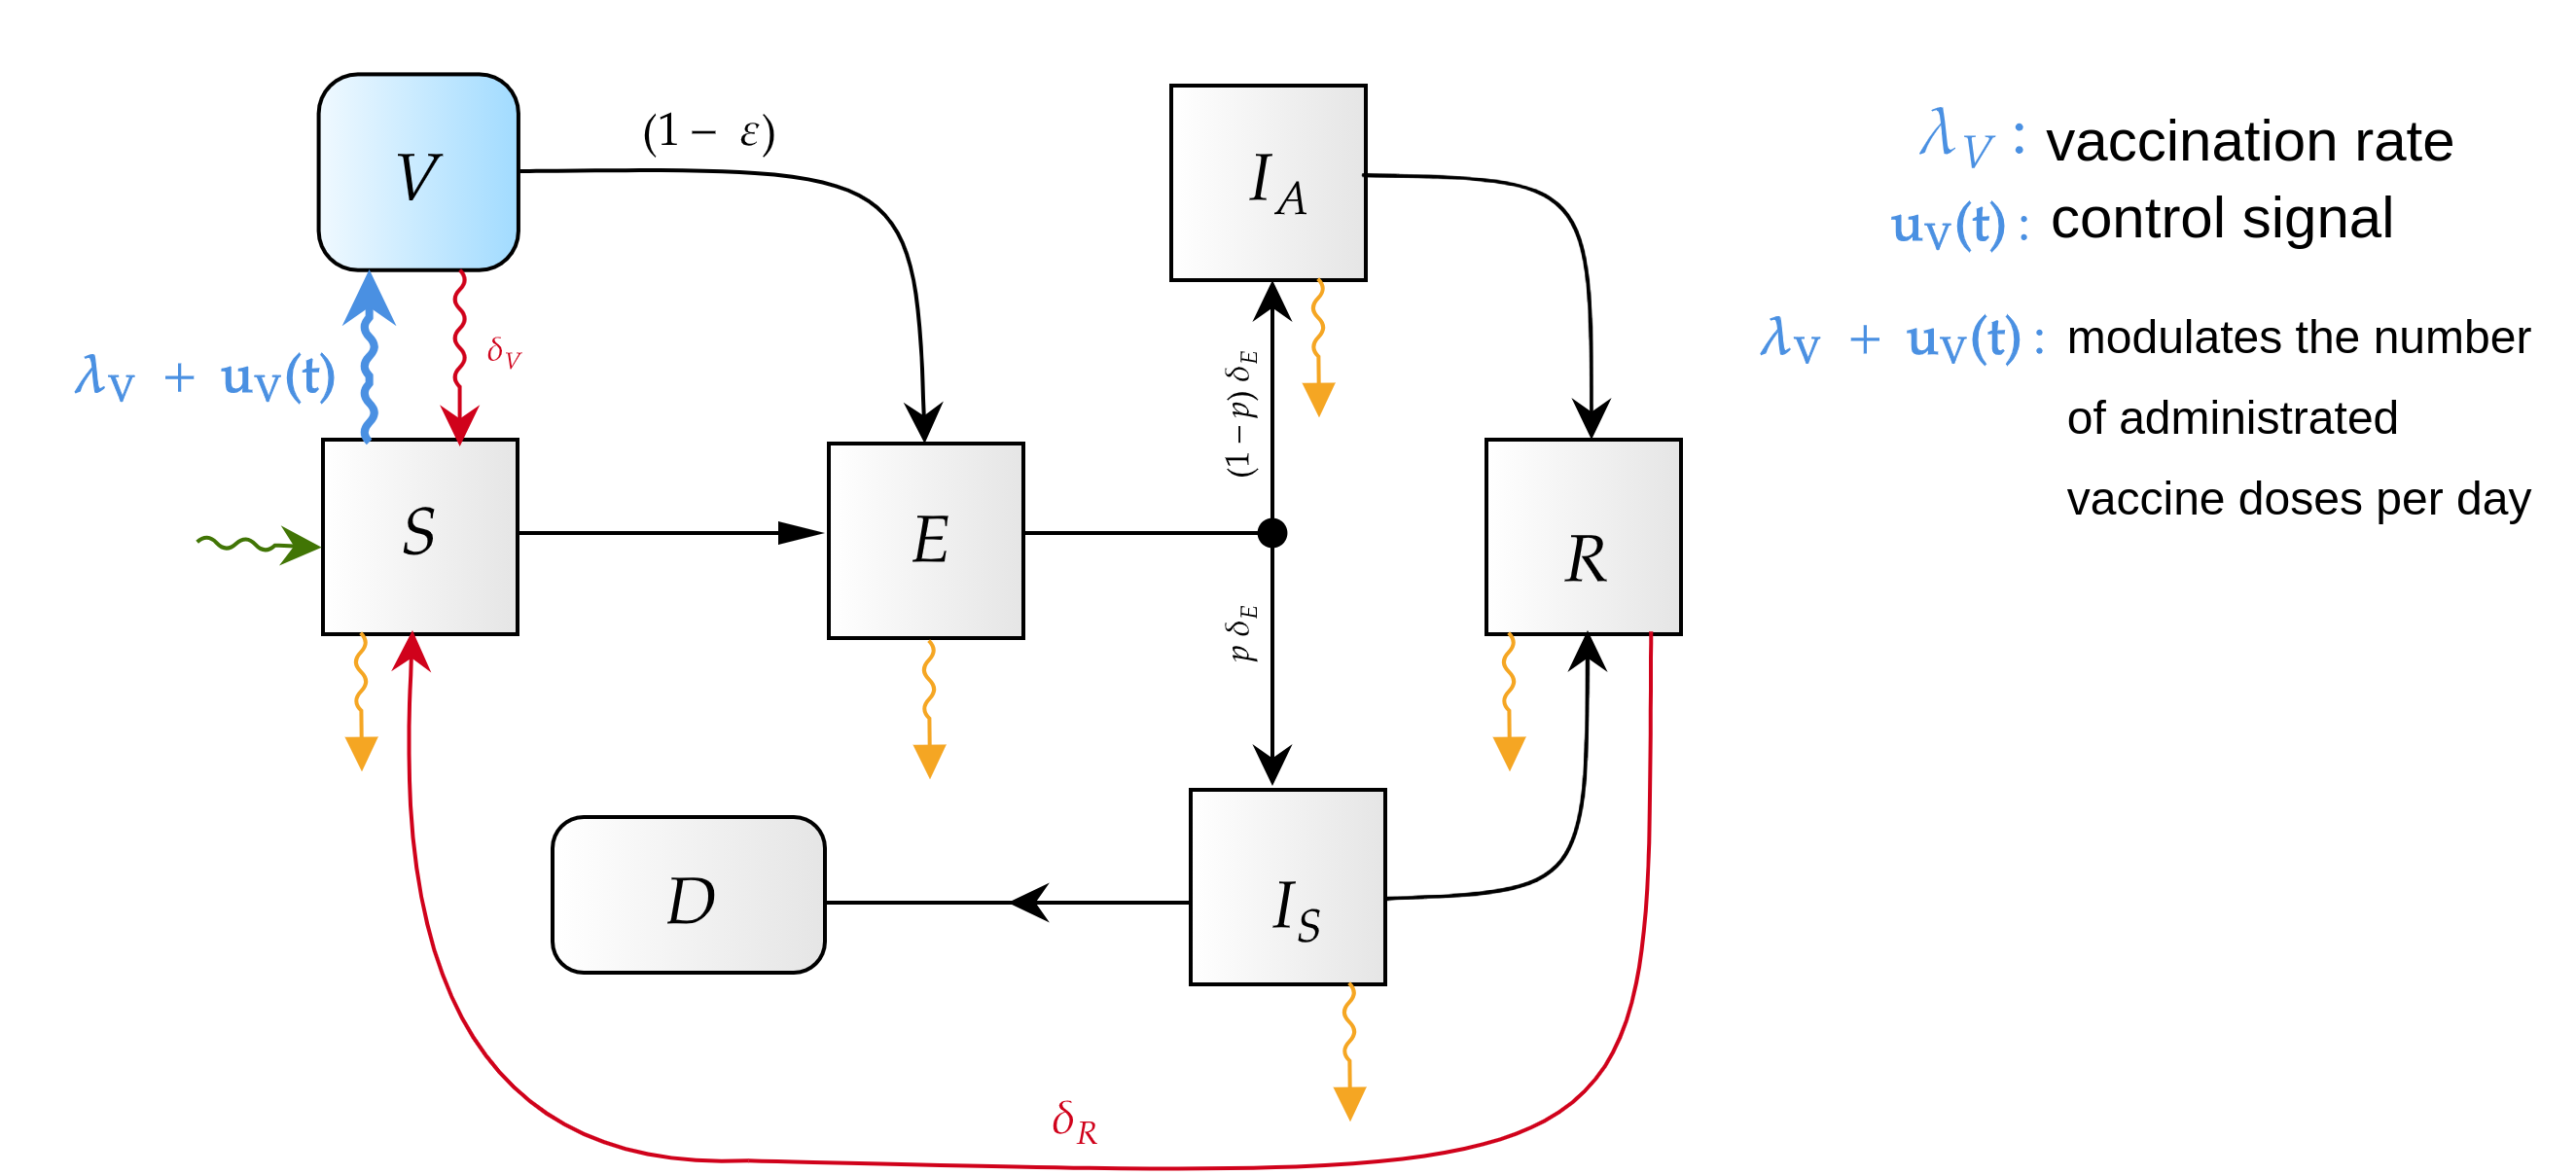
\includegraphics[scale=.125,%
                keepaspectratio]{assets/SchemeModel01.png}
        }
        \only<3>{
            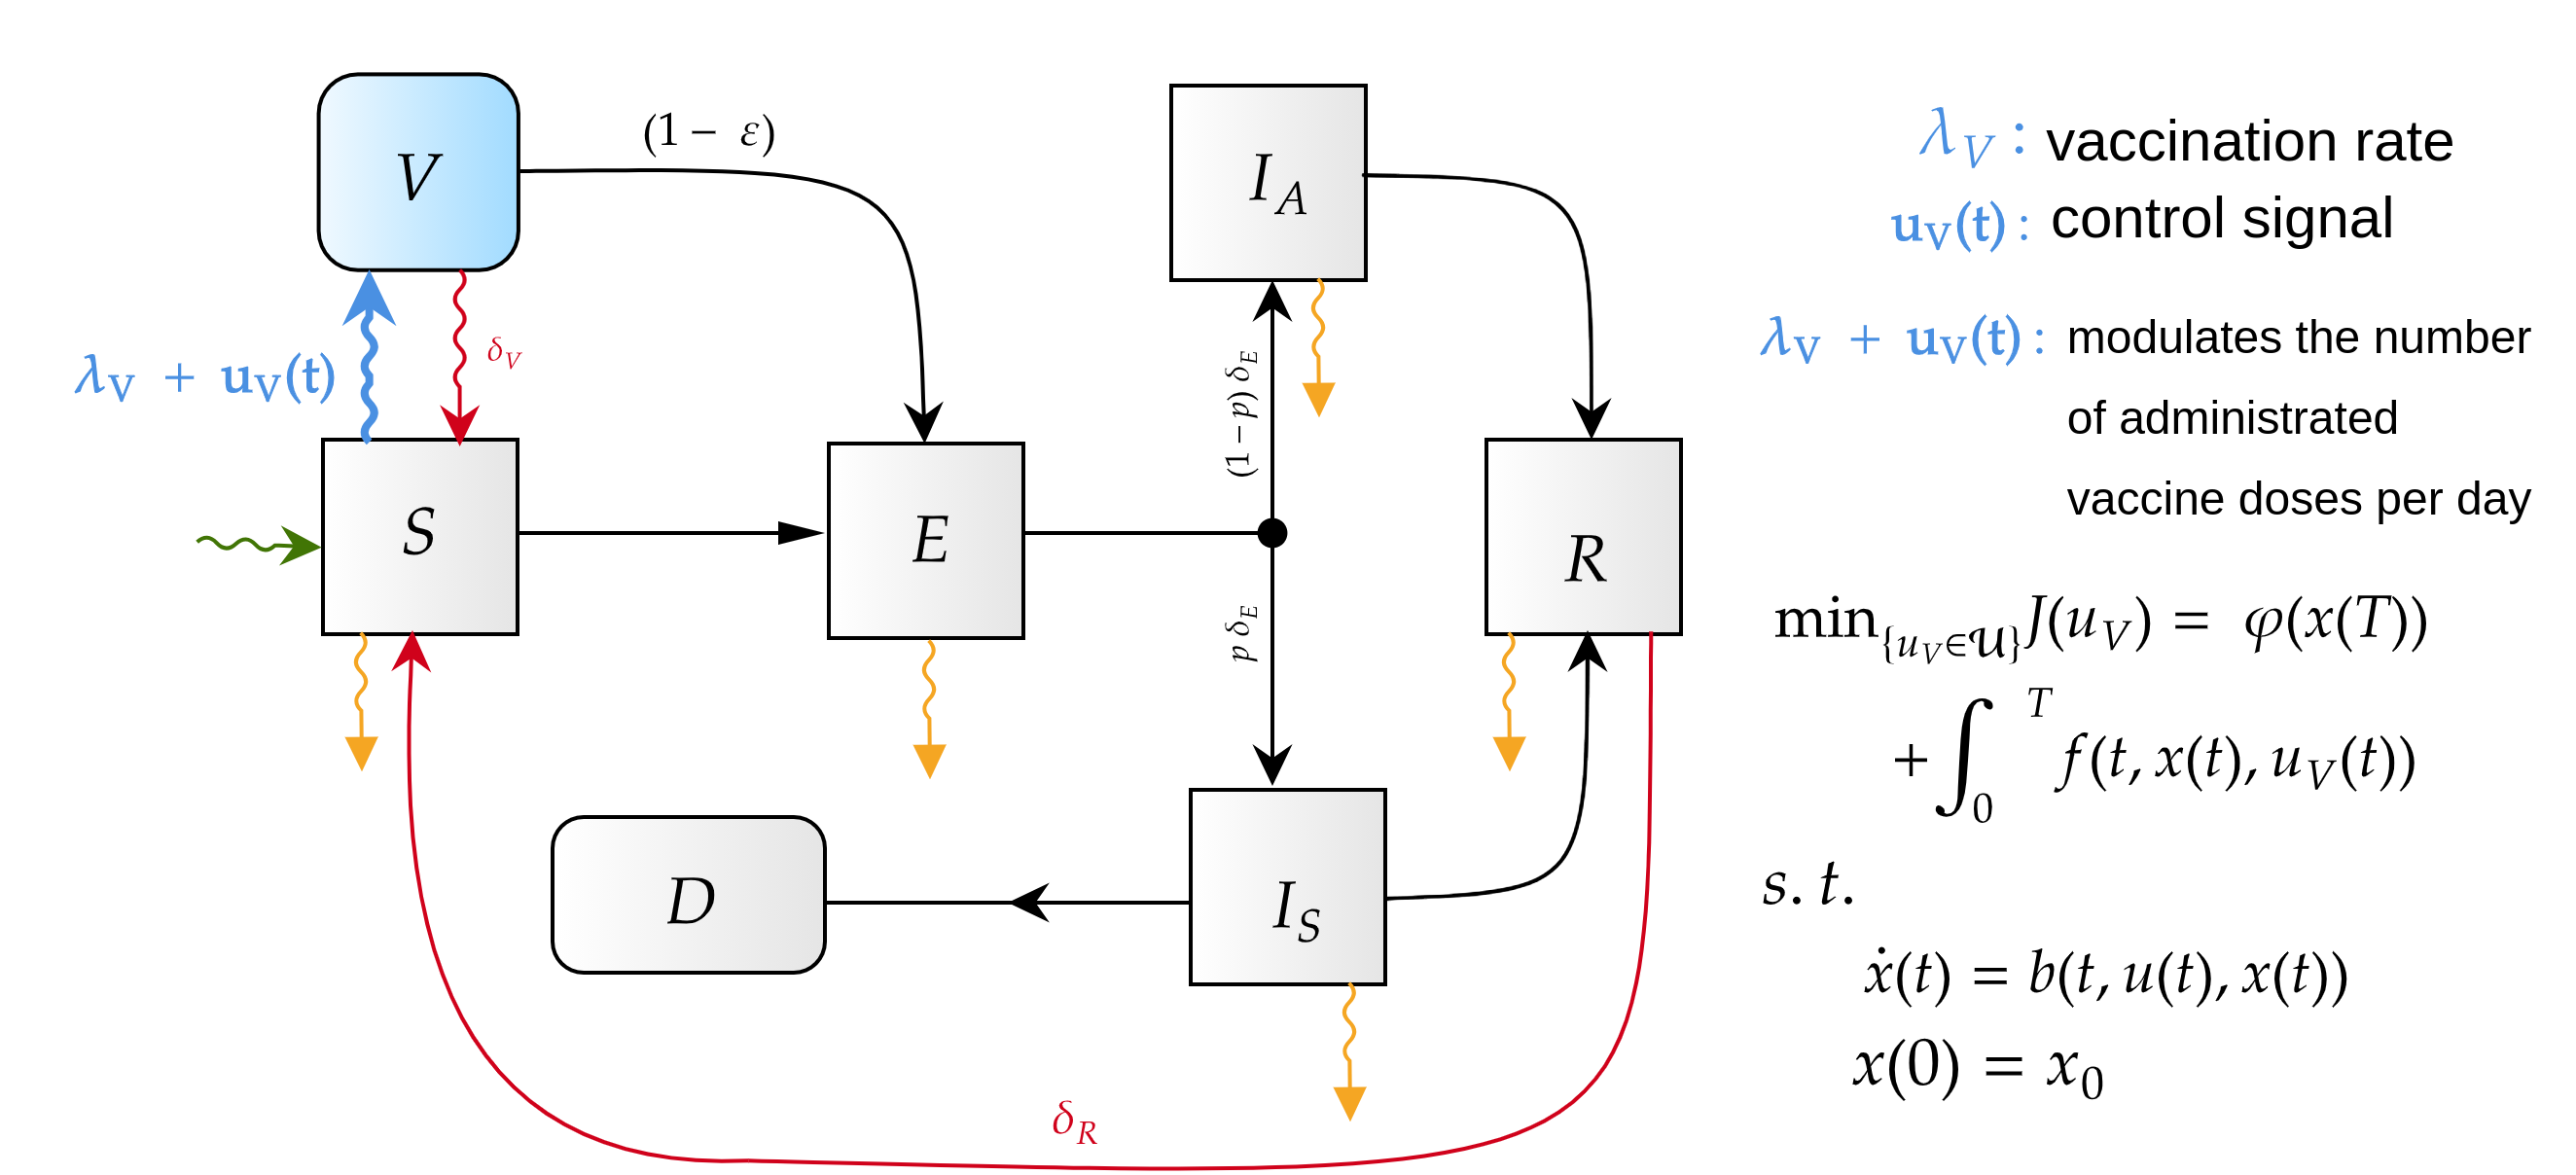
\includegraphics[scale=.125,%
                keepaspectratio]{assets/SchemeModel02.png}
        }
    \end{textblock*}
\end{frame}
\begin{frame}{The disability-adjusted life year (DALY)}
    \begin{textblock*}{120mm}(5mm,10mm)
        %
        \begin{graybox}{{$DALY(c,s,a,t) = YLL(c,s,a,t) + YLD(c,s,a,t)$}}
            For given cause c, age a, sex s and year t
            \begin{description}
                \item[$YLL:$] Years of life lost due to premature death.
                    $$
                        YLL(c,s,a,t) = N(c,s,a,t) \times L(s,a)
                    $$
                    \begin{itemize}
                         \item
                             $N(c,s,a,t):$ is the number of 
                             deaths due to the cause $c$ 
                         \item
                             $L(s,a):$ is a standard loss 
                             function specifying years of life lost 
                    \end{itemize}
                 \item[$YLD:$] Years of life list due to disability   
                     $$
                         YLD(c,s,a,t) = I(c,s,a,t) \times DW(c,s,a) 
                         \times L(c,s,a,t)
                     $$
                    \begin{itemize}
                        \item
                            $I(c,s,a,t):$ number of incident cases for cause c
                        \item
                            $DW(c,s,a):$ disability weight for cause c
                        \item
                            $L(c,s,a,t):$  average duration of the case 
                            until remission or death (years)
                    \end{itemize}
            \end{description}
       \end{graybox}
       \begin{equation*}
            \begin{aligned}
             & \only<2->{\min_{u_V  \in \mathcal{U}[0, T]}}
             J(u_V) :=
             \only<3->{
                \underbrace{a_D ( D(T) - D(0))}_{:=YLL}  +
                \underbrace{a_S (Y_{I_S}(T) - Y_{I_S}(0))}_{:=YLD}
             }
            \end{aligned}
       \end{equation*}        
    \end{textblock*}
    \end{frame}
    %
    %
    \begin{frame}{Optimal Control Problem}
    \begin{textblock*}{120mm}(10mm,10mm)
        \only<1-3>{
            \begin{equation*}
                    \begin{aligned}
                             &
                             \textcolor<1>{orange}{%
                                \min_{u_V  \in \mathcal{U}[0, T]}
                                J(u_V) :=
                                    \underbrace{a_D ( D(T) - D(0))}_{:=YLL}  +
                                    \underbrace{
                                        a_S (Y_{I_S}(T) - Y_{I_S}(0))
                                    }_{:=YLD}
                            }
                        \\
                             & 
                             \textcolor<2>{orange}{
                                u_V(\cdot)   \in [u_{\min}, u^{\max}],
                            }
                        \\
                            &
                            \textcolor<3>{orange}{
                                \kappa I_S(t)  
                                \leq B, \quad \forall t \in [0, T],
                             }
                        %}
                    \end{aligned}
            \end{equation*}
        }
    \end{textblock*}    
    \begin{textblock*}{85mm}(0mm,10mm)        
        \only<4->{
            \begin{equation*}
                \begin{aligned}
                    &\min_{u_V  \in \mathcal{U}[0, T]}
                    J(u_V) :=
                    %\int_0 ^ T
                    % a_D D(s) + a_S Y_{I_S}(s) ds
                    a_D ( D(T) - D(0)) +
                    a_S (Y_{I_S}(T) - Y_{I_S}(0))
                    \\
                    \text{s.t.} &
                    \\
                    &f_{\lambda}
                    :=
                    \frac{\beta_S I_S + \beta_AI_A}{\bar{N}}
                    \\
                    S'(t)
                    &=
                    \mu \bar{N} + \delta_V V + \delta_R R
                    \\
                    &-
                    (f_{\lambda} + \mu + \lambda_V +  u_V(t)) S
                    \\
                    E'(t)
                    &=
                    f_{\lambda} (S + (1-\epsilon) V)
                    - (\mu+\delta_E) E
                    \\
                    I'_S(t)
                    &=p
                    \delta_E
                    E-(\mu + \alpha_S) I_S
                    \\
                    I'_A(t)
                    &= (1 - p) \delta_E E-(\mu + \alpha_A) I_A
                    \\
                    R'(t)
                    &= (1 - \theta) \alpha_S I_S + \alpha_A I_A
                    - (\mu + \delta_R) R
                    \\
                    D'(t)&=
                    \theta \alpha_S I_S
                    \\
                    V'(t)&=
                    (\lambda_V + u_V(t)) S -
                    \left(
                    (1 -\epsilon) f_{\lambda} V +
                    \mu + \delta_V
                    \right) V
                    \\
                    X'(t)&=
                    (\lambda_V + u_V(t))(S + E + I_A + R)           
                \end{aligned}
            \end{equation*}
        }
    \end{textblock*}
%
    \begin{textblock*}{60mm}(70mm, 30mm)
        \only<4->{
            \begin{equation*}
                \begin{aligned}
                    S(0) &= S_0, \ E(0) = E_0, \ I_S(0) = I_{S_{0}},
                    \\
                    I_A(0) &= I_{A_{0}}, \ R(0) = R_0, \ D(0) = D_0,
                    \\
                    V(0) &= 0, \ X(0) = 0, \ X(T) = x_{coverage},
                    \\
                    u_V(\cdot) & \in [u_{\min}, u^{\max}],
                    \\
                    \kappa I_S(t) & \leq B, \quad \forall t \in [0, T],
                    \\
                    \bar{N}(t) &= S + E + I_S + I_A + R + V.
                \end{aligned}
            \end{equation*}
        }
    \end{textblock*}
\end{frame}